\documentclass{beamer}
% listings-csharp.tex

\usepackage{listings}
\usepackage{xcolor}

\lstdefinelanguage{CSharp}{
  morekeywords={
    abstract, as, base, bool, break, byte, case, catch, char, checked, class, const, continue,
    decimal, default, delegate, do, double, else, enum, event, explicit, extern, false, finally,
    fixed, float, for, foreach, goto, if, implicit, in, int, interface, internal, is, lock, long,
    namespace, new, null, object, operator, out, override, params, private, protected, public,
    readonly, ref, return, sbyte, sealed, short, sizeof, stackalloc, static, string, struct,
    switch, this, throw, true, try, typeof, uint, ulong, unchecked, unsafe, ushort, using,
    virtual, void, volatile, while, async, await, var, dynamic
  },
  sensitive=true,
  morecomment=[l]{//},
  morecomment=[s]{/*}{*/},
  morestring=[b]",
}

% Optional: set global lstlisting defaults here
\lstset{
  basicstyle=\ttfamily\footnotesize,
  keywordstyle=\color{blue},
  commentstyle=\color{gray},
  stringstyle=\color{orange},
  emph={Draw, Main, Console, WriteLine, Cards, DrawCardPreview},
  emphstyle=\color[rgb]{0,0.6,0}\bfseries,
  breaklines=true,
  breakatwhitespace=false,
  numbers=left,
  numberstyle=\tiny\color{gray},
  numbersep=10pt,
  showstringspaces=false
}

\usepackage{graphicx}
\usepackage{tikz}
\usepackage{multicol}
\usepackage{listings}
\usepackage{pgfgantt}
\usepackage{xcolor}
\usepackage[utf8]{inputenc}
\setbeamertemplate{footline}[frame number]
\graphicspath{ {./images/} }

\lstdefinelanguage{yaml}{
  keywords={true,false,null,y,n},
  sensitive=false,
  comment=[l]{\#},
  morecomment=[s]{/*}{*/},
  morestring=[b]',
  morestring=[b]"
}
\lstset{
  basicstyle=\ttfamily\small,
  columns=fullflexible,
  language=yaml,
  breaklines=true,
  frame=single,
  literate={ä}{{\"a}}1 {ö}{{\"o}}1 {ü}{{\"u}}1
           {Ä}{{\"A}}1 {Ö}{{\"O}}1 {Ü}{{\"U}}1
           {ß}{{\ss}}1
}

\lstdefinelanguage{Dockerfile}{
  keywords={FROM, RUN, CMD, LABEL, MAINTAINER, EXPOSE, ENV, ADD, COPY, ENTRYPOINT, VOLUME, USER, WORKDIR, ARG, ONBUILD, STOPSIGNAL, HEALTHCHECK, SHELL},
  sensitive=true,
  morecomment=[l]{\#},
  morestring=[b]",
}
\lstset{
  basicstyle=\ttfamily\small,
  keywordstyle=\color{blue}\bfseries,
  commentstyle=\color{gray},
  stringstyle=\color{orange},
  showstringspaces=false,
  breaklines=true,
  frame=single,
}

\lstdefinelanguage{CSharp}{
  morekeywords={
    abstract, as, base, bool, break, byte, case, catch, char, checked, class, const, continue,
    decimal, default, delegate, do, double, else, enum, event, explicit, extern, false, finally,
    fixed, float, for, foreach, goto, if, implicit, in, int, interface, internal, is, lock, long,
    namespace, new, null, object, operator, out, override, params, private, protected, public,
    readonly, ref, return, sbyte, sealed, short, sizeof, stackalloc, static, string, struct, switch,
    this, throw, true, try, typeof, uint, ulong, unchecked, unsafe, ushort, using, virtual, void,
    volatile, while, var, dynamic, get, set, value, await, async, partial, yield
  },
  sensitive=true,
  morecomment=[l]{//},
  morecomment=[s]{/*}{*/},
  morestring=[b]",
  morestring=[b]',
}

\title{WaterWizards}
\author{Justin Dewitz, Erick Zeiler, Max Kondratov, Julian <Nachname>}
\date{17. Juli 2025}

\begin{document}

\begin{frame}[plain]
  \titlepage
  \begin{tikzpicture}[remember picture,overlay]
    \node[anchor=south west, xshift=0.2cm, yshift=0.2cm] at (current page.south west) {
\includegraphics[height=2.5cm]{wizblu.png}};
    \node[anchor=south east, xshift=-0.2cm, yshift=0.2cm] at (current page.south east) {
\includegraphics[height=2.5cm]{wizred.png}};
  \end{tikzpicture}
\end{frame}

\begin{frame}
\frametitle{Inhaltsverzeichnis}
\tableofcontents[hideallsubsections] \small
\end{frame}

\section{Einleitung}
\begin{frame}
\frametitle{Einleitung}
\begin{itemize}
  \item Was ist WaterWizards?
  \begin{enumerate}
    \item Mulitplayer Real-Time Schiffe versenken
    \item Angriff durch Zauber, die durch Karten repräsentiert werden
    \item Ziel: Zerstörung der gegnerischen Schiffe
  \end{enumerate}
  \item Warum WaterWizards?
  \begin{enumerate}
    \item Schiffe versenken ist ein Klassiker
    \item Durch Real-Time wird es dynamischer
    \item Für jede Altersgruppe interessant
  \end{enumerate}
  \item Was macht WaterWizards besonders?
    \begin{enumerate}
      \item Kombination aus Strategie und schnellen Entscheidungen
      \item Zauber und Karten bringen neue Dynamik ins Spiel
      \item Multiplayer und Echtzeit sorgen für Spannung
    \end{enumerate}
  \item Für wen ist das Spiel gedacht?
    \begin{enumerate}
      \item Strategie-Fans
      \item Familien und Freunde
      \item Alle Altersgruppen
    \end{enumerate}
\end{itemize}
\end{frame}

\section{Organisation}
\begin{frame}
  \frametitle{Organisation}
  \begin{itemize}
    \item git über GitHub für die Versionsverwaltung 
    \item Scrum mit 2-Wochen-Sprints
    \item Kanban/Issue-Board über GitHub
    \item Kommunikation über Discord-Server
  \end{itemize}
\end{frame}

\subsection{Backlog}
\begin{frame}
\frametitle{Backlog}
  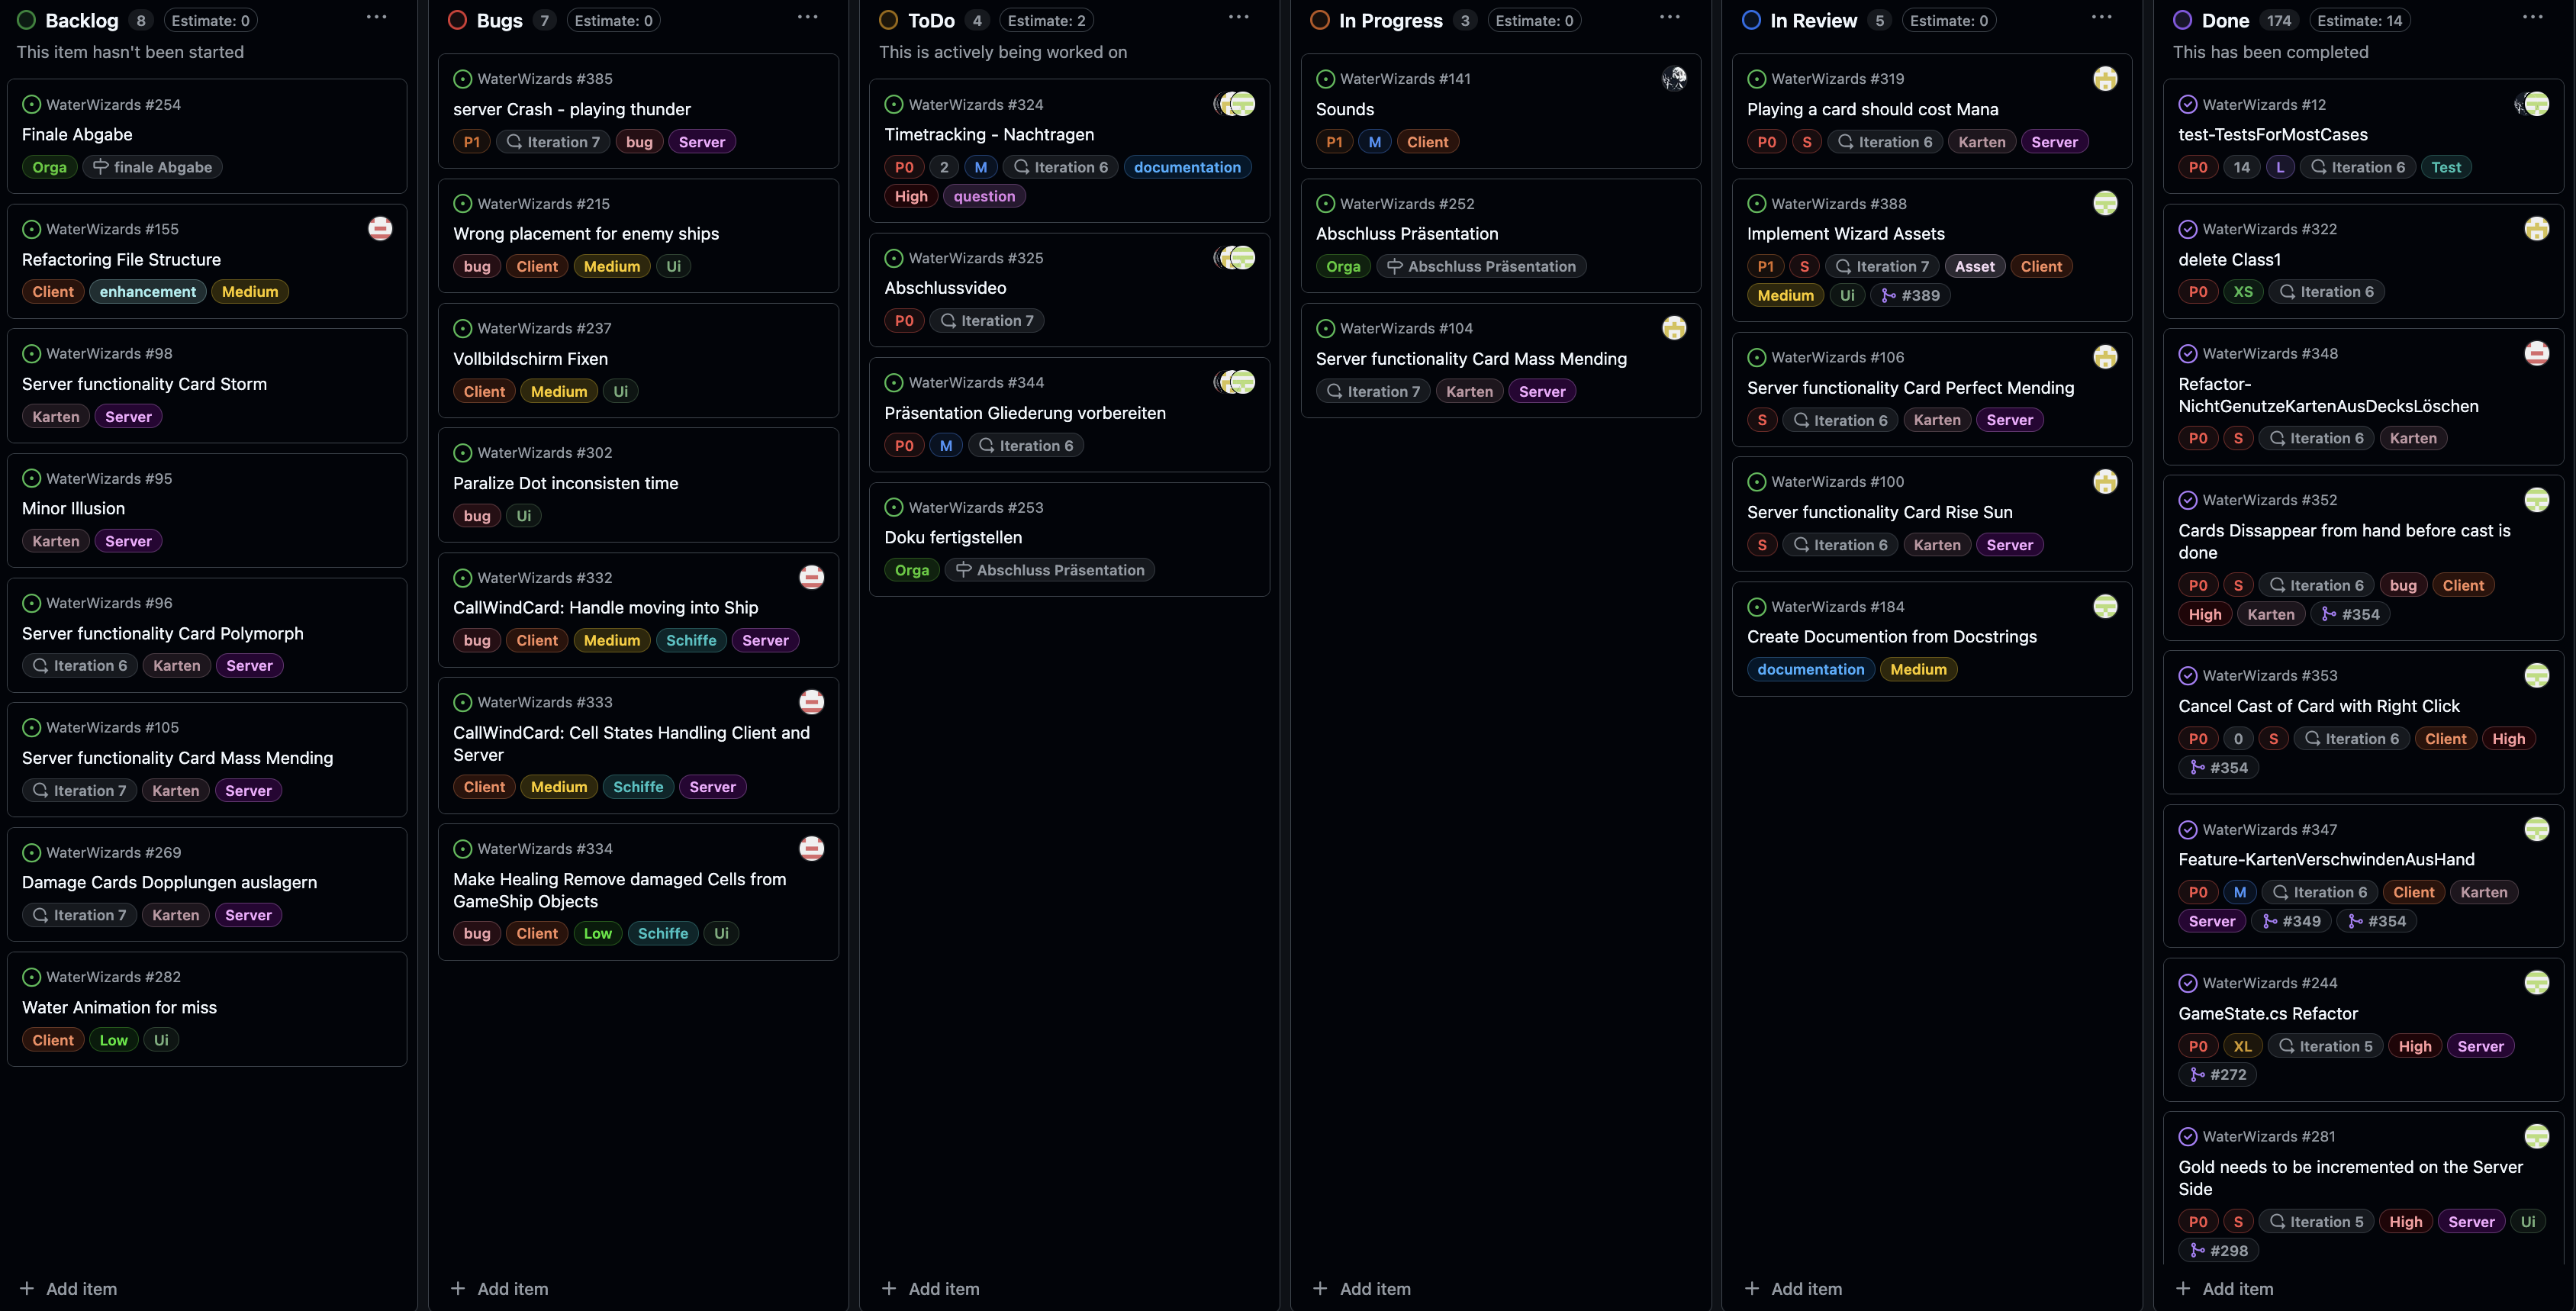
\includegraphics[width=\textwidth]{Kanban.png}
\end{frame}

\subsection{Projektplan}
\begin{frame}
\frametitle{Projektplan}
\begin{center}
\resizebox{\textwidth}{!}{
  \begin{ganttchart}[
    y unit chart=0.3cm,
    vgrid,
    hgrid,
    bar/.append style={fill=blue!40},
    group/.append style={fill=orange!60},
    milestone/.append style={fill=red!80},
    group label font=\bfseries\scriptsize,
    bar label font=\scriptsize,
    milestone label font=\scriptsize,
    title label font=\scriptsize
  ]{1}{14}
    \gantttitle{Wochen}{14} \\
    \gantttitlelist{1,...,14}{1} \\

    \ganttgroup{Prototyp}{1}{3} \\
    \ganttbar{Anforderungsanalyse}{1}{1} \\
    \ganttbar{Architektur \& Server Logic}{1}{2} \\
    \ganttbar{UI}{2}{2} \\

    \ganttgroup{Design \& Erste Karten + MVP}{3}{6} \\
    \ganttbar{UI Design}{3}{3} \\
    \ganttbar{3 Attack Karten}{4}{4} \\
    \ganttbar{Showcase MVP vorbereiten}{4}{6} \\

    \ganttgroup{Testen}{5}{12} \\
    \ganttbar{Unit Tests}{5}{11} \\
    \ganttbar{1 Integrationstests}{12}{12} \\

    \ganttgroup{Zielgenaue Implementierung}{6}{10} \\
    \ganttbar{Backend - Frontend Kommunikation verbessern}{5}{8} \\
    \ganttbar{Frontend Feinschliff}{6}{10} \\
    \ganttbar{Refactoring für bessere Lesbarkeit}{7}{9} \\

    \ganttgroup{Abschluss}{13}{14} \\
    \ganttbar{Dokumentation}{13}{13} \\
    \ganttbar{Präsentation}{14}{14} \\
    \ganttbar{Projekt Feinschliff}{13}{14} \\
    \ganttmilestone{Projekt Abgabe}{14}
  \end{ganttchart}
}
  \vspace{0.4em}
  {\scriptsize
    \begin{tabular}{@{}ll}
      \textcolor{orange!60}{\rule{0.5em}{0.5em}} & Projektphase (Gruppe) \\
      \textcolor{blue!40}{\rule{0.5em}{0.5em}} & Aufgabe (Task) 
    \end{tabular}
  }
\end{center}
\end{frame}

\section{Rollen des Projektes}
\begin{frame}
  \begin{itemize}
    \item Architektur: Justin Dewitz
    \item Dokumentation: Erick Zeiler
    \item Code-Qualität: Paul Schneider (abgesprungen)
    \item Git Repository: Max Kondratov
  \end{itemize}
\frametitle{Rollen des Projektes}

\end{frame}

\subsection{Ansprechpartner}
\begin{frame}
\frametitle{Ansprechpartner}

\end{frame}

\section{Technologie + Architektur}
\begin{frame}
\frametitle{Technologie + Architektur}
  \begin{itemize}
    \item Programiersprache: C\#
    \item Raylib für die grafische Darstellung
    \item LiteNetLib für die Client-Server-Verbindung
    \item Nuke für das Build-System
    \item CodeQl für die statische Code-Analyse
    \item GitHub Actions für die CD-Pipeline
    \item GitHub Pages für die Dokumentation
    \item Event-Driven Architektur
    \item Docker für die Containerisierung
    \item Hetzner Server für das Hosting
  \end{itemize}
\end{frame}

\begin{frame}
  \frametitle{Spiel-Bildschirm / GameScreen}
  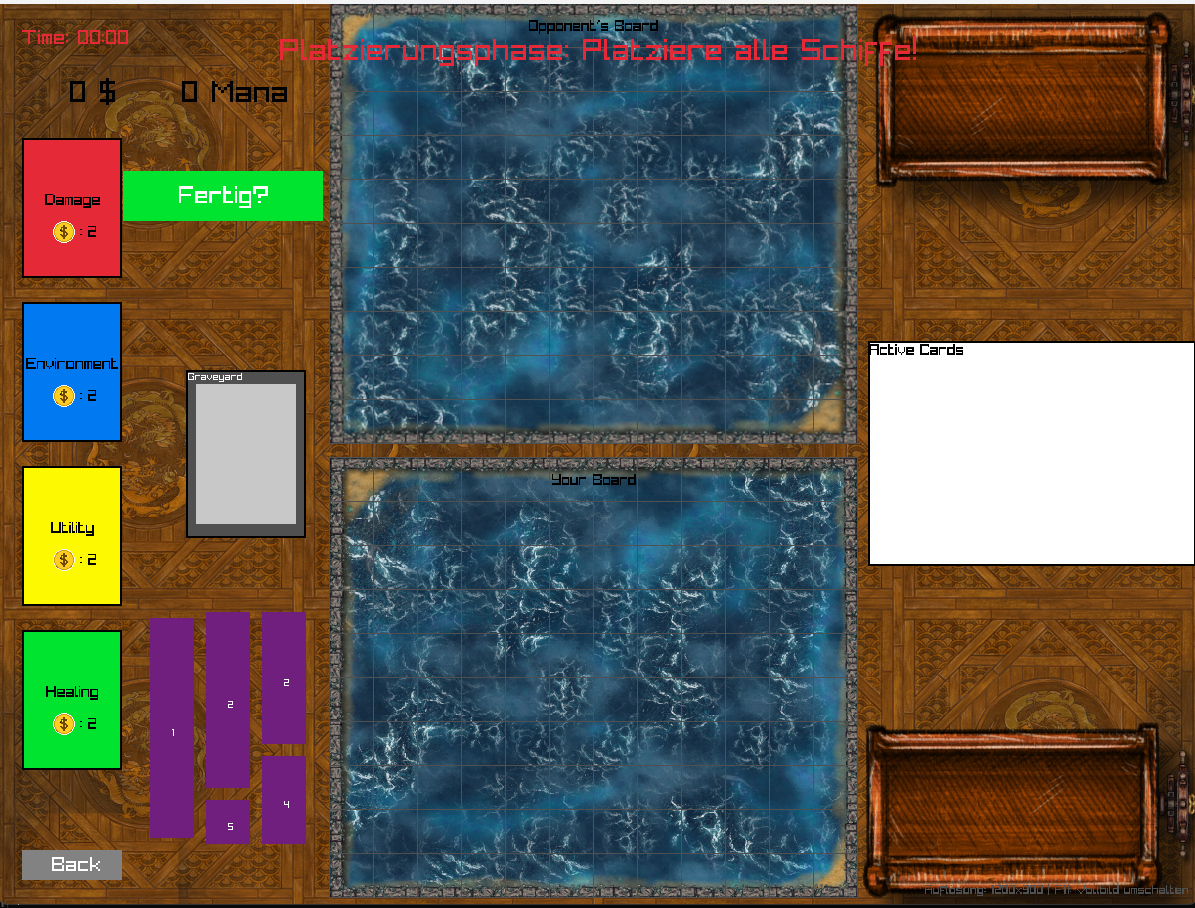
\includegraphics[width=\textwidth]{GameScreen.png}
\end{frame}

\subsection{UI}
\begin{frame}
  \frametitle{UI}
  \begin{itemize}
    \item Raylib für die grafische Darstellung
    \item Grafische Darstellung getrennt von Spielfunktionalität:
      \begin{itemize}
        \item Client übernimmt das Anzeigen und Handhabung des User Interfaces 
      \end{itemize}
    \item Gemeint sind Interaktive dargestellte Elemente, z.B:
    \begin{itemize}
      \item Die Kartenstapel, die Schiffe oder die Kartenhand
    \end{itemize}
    \item Alle Elemente werden durch eine Methode Draw angezeigt, welche in der GameLoop ausgeführt wird.
    \item Die wenige Logik, die auf dem Client ausgeführt wird, wird in diesen Draw Methoden ausgeführt
  \end{itemize} 
\end{frame}

\subsection{UI-Example}
\begin{frame}[fragile]
  \frametitle{UI-Beispiel aus der GameHand Klasse}
  \begin{lstlisting}[language=CSharp, basicstyle=\ttfamily\tiny, breaklines=true]
    public virtual void Draw(bool front)
    { 
        int availableHandWidth = (int)(ScreenWidth * 0.2f);
        int totalCardWidth = Cards.Count * CardWidth;
        int excess = totalCardWidth - availableHandWidth;
        int offset = excess > 0 ? excess / Cards.Count : 0;
        for (int i = 0; i < Cards.Count; i++)
        {
            //[...]

            Cards[i].Draw(centralX + cardX, cardY, front);

            DrawCardPreview(front, i, cardX, effectiveCardWidth);
        }
    }
  \end{lstlisting}
\end{frame}

\begin{frame}
  \frametitle{UI Struktur GameScreen}
  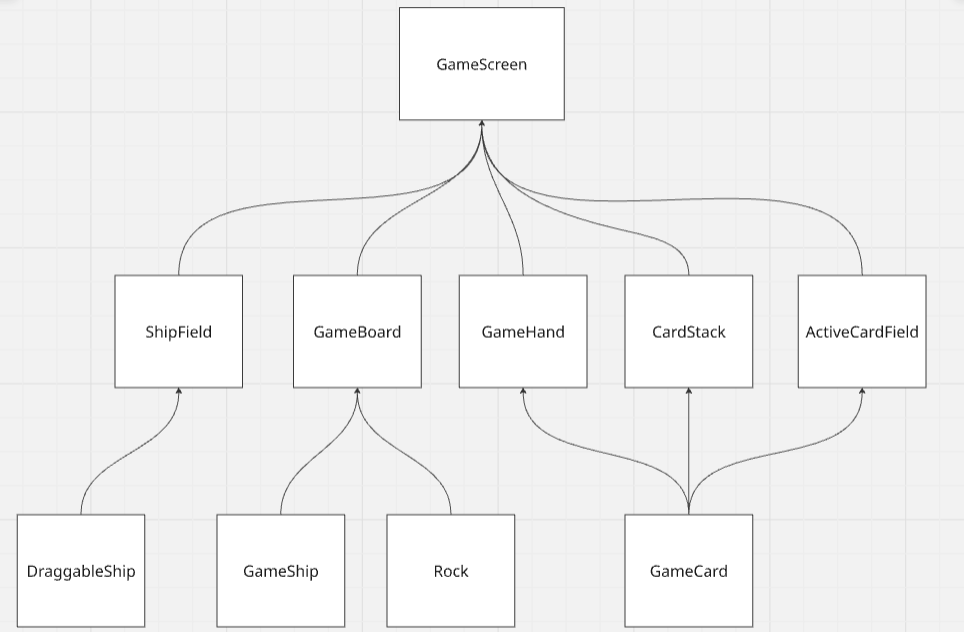
\includegraphics[width=\textwidth]{UI-Struktur.png}
\end{frame}

\subsection{TextureManager}
\begin{frame}[fragile]
\frametitle{TextureManager}
\begin{lstlisting}[language=CSharp, basicstyle=\ttfamily\tiny, breaklines=true]
/// <summary>
/// Verwaltet das Laden und Entladen von Texturen für das Spiel.
/// </summary>
public class TextureManager
{
    private static List<Texture2D> textures = [];

    /// <summary>
    /// Lädt eine Textur aus einer Datei und speichert sie für späteres Entladen.
    /// </summary>
    /// <param name="file">Pfad zur Texturdatei</param>
    /// <returns>Die geladene Textur als <see cref="Texture2D"/></returns>
    public static Texture2D LoadTexture(string file)
    {
        var texture = Raylib.LoadTexture(file);
        textures.Add(texture);
        return texture;
    }

    /// <summary>
    /// Entlädt alle zuvor geladenen Texturen aus dem Speicher.
    /// </summary>
    public static void UnloadAllTextures()
    {
        foreach (var texture in textures)
        {
            Raylib.UnloadTexture(texture);
        }
    }
}
\end{lstlisting}
\end{frame}

\subsection{Server/Backend}
\begin{frame}
\frametitle{Server/Backend}
  \begin{itemize}
    \item Das Backend ist in C\# mit der Library LiteNetLib geschrieben
    \item Ein globaler Server der eine Lobby auf Hetzner bereitstellt
    \item Server wird in Docker-Containern ausgeführt
    \item Der Server wird auf dem Port 7777/UDP bereitgestellt
  \end{itemize}
\end{frame}

\subsection{GameState}
\begin{frame}[fragile]
  \frametitle{Spielzustand / GameState}
  \begin{itemize}
    \item Programm wird in Zustands-Klassen (States) beschrieben
    \item Spiel wird in der GameState-Klasse beschrieben
  \end{itemize}
  \textbf{Ausschnitt: }
  \begin{lstlisting}
    public class GameState
    {
      public NetPeer[] players = new NetPeer[2];
      public static readonly int boardWidth = 12;
      public static readonly int boardHeight = 10;
      public readonly Cell[][,] boards = new Cell[2][,];
      public Cell[,] Player1 => boards[0];
      public Cell[,] Player2 => boards[1];
      public readonly List<Cards>[] hands;
      private readonly NetManager server;
      public readonly ServerGameStateManager manager;
      public List<Cards> Player1Hand => hands[0];
      public List<Cards> Player2Hand => hands[1];
      public static List<Cards>? ActiveCards //[...]
      public static List<Cards>? UtilityStack //[...]
  \end{lstlisting}
\end{frame}

\subsection{Factory Pattern}
\begin{frame}[fragile]
\frametitle{Factory Pattern}
  \begin{itemize}
    \item Das Factory-Pattern wird für die Erstellung von Kartenobjekten verwendet
    \item Für jede Kartenart gibt es eine eigene Factory
  \end{itemize}
  
  \textbf{Beispiel: DamageCardFactory}
  \begin{lstlisting}[language=CSharp, basicstyle=\ttfamily\tiny, breaklines=true]
    public static class DamageCardFactory 
    {
        public static IDamageCard Create(CardVariant variant) 
        {
            return variant switch 
            {
                CardVariant.Firebolt => new FireboltCard(),
                CardVariant.FrostBolt => new FrostBoltCard(),
                CardVariant.Lightning => new LightningCard(),
                _ => throw new ArgumentException($"Unknown variant: {variant}")
            };
        }
    }
  \end{lstlisting}
  
  \textbf{Vorteile:}
  \begin{itemize}
    \item Neue Karten können einfach ergänzt werden
    \item Spiellogik bleibt unverändert
    \item Klare Trennung von Erstellung und Verwendung
  \end{itemize}
\end{frame}

\subsection{Shared}
\begin{frame}
\frametitle{Shared}
  \begin{itemize}
    \item Shared enthält alle Klassen, die sowohl im Client als auch im Server verwendet werden
    \item Enthält die Definitionen der Karten und der Kartentypen
    \item Enthält die Definitionen der Schiffe und der Schiffs-Typen
  \end{itemize}
\end{frame}

\subsection{Backend - Client Kommunikation}
\begin{frame}
\frametitle{Backend - Client Kommunikation}
\begin{columns}
  \begin{column}{0.45\textwidth}
    Event-Driven Architektur
    \begin{itemize}
      \item UDP für die Echtzeit-Kommunikation
      \item Nachrichten basiertes Protokoll für beidseitige Kommunikation
    \end{itemize}
  \end{column}
  \begin{column}{0.55\textwidth}
    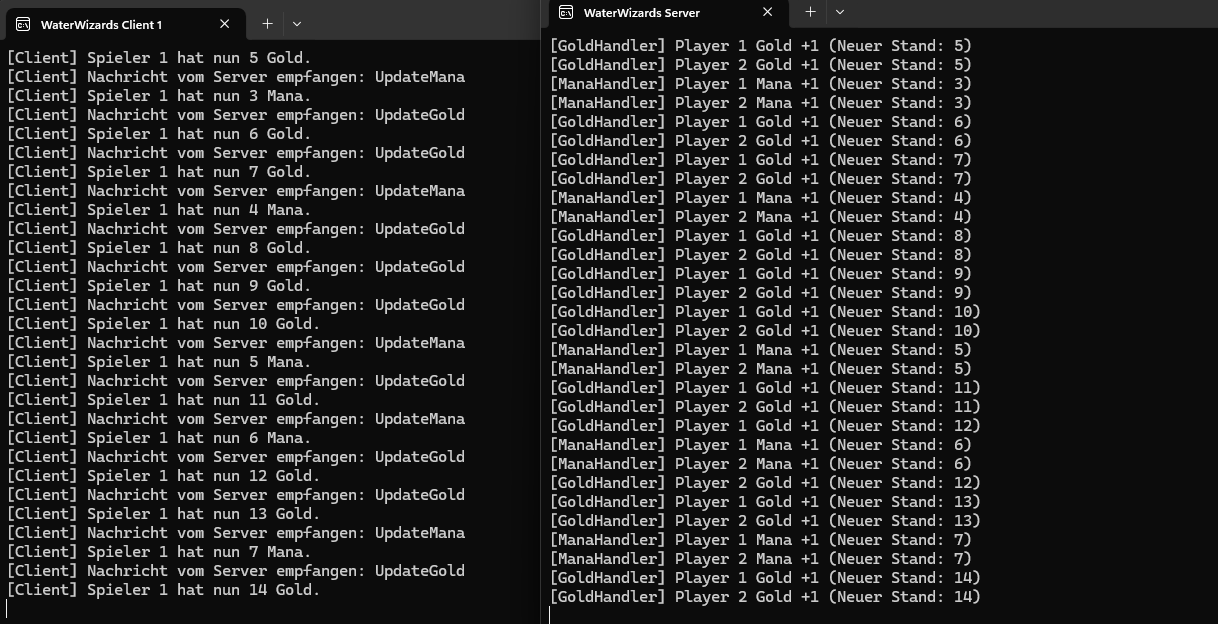
\includegraphics[width=\textwidth]{Server-Client-Logs.png}
  \end{column}
\end{columns}
\end{frame}

\subsection{Nachrichtenempfang + Parsing im Client}
\begin{frame}[fragile]
\frametitle{Nachrichtenempfang + Parsing im Client}
  \begin{lstlisting}[language=CSharp, basicstyle=\ttfamily\tiny, breaklines=true]
     private void HandleClientReceiveEvent(
        NetPeer peer,
        NetPacketReader reader,
        byte channelNumber,
        DeliveryMethod deliveryMethod
    )
    {
        try
        {
            string messageType = reader.GetString();
            Console.WriteLine($"[Client] Nachricht vom Server empfangen: {messageType}");

            switch (messageType)
            {
                case "UpdatePauseState":
                    bool isPaused = reader.GetBool();
                    if (isPaused)
                    {
                        GameStateManager.Instance.GetGamePauseManager().PauseGame();
                    }
                    else
                    {
                        GameStateManager.Instance.GetGamePauseManager().ResumeGame();
                    }
                    break;
                case "StartGame":
                    GameStateManager.Instance.SetStateToInGame();
                    break;
                ...
          }
          ...
    }
  \end{lstlisting}
\end{frame}

\section{DevOps}
\begin{frame}
\frametitle{DevOps}
  \begin{itemize}
    \item CI-Pipeline
    \item CD-Pipeline
    \item Statische Code-Analyse
    \item Pull Requests mit 4-Augen Prinzip
    \item Dokumentation auf Github Pages
  \end{itemize}
\end{frame}

\subsection{CI/CD Pipeline}
\begin{frame}
\frametitle{CI/CD Pipeline}
  \begin{multicols}{2}
    \begin{itemize}
      \item \textbf{CI}
        \begin{itemize}
          \item Nuke build für die Continous-Integration
          \item dotnet \textit{restore, build, test}, werden bei jedem PR ausgeführt
        \end{itemize}
      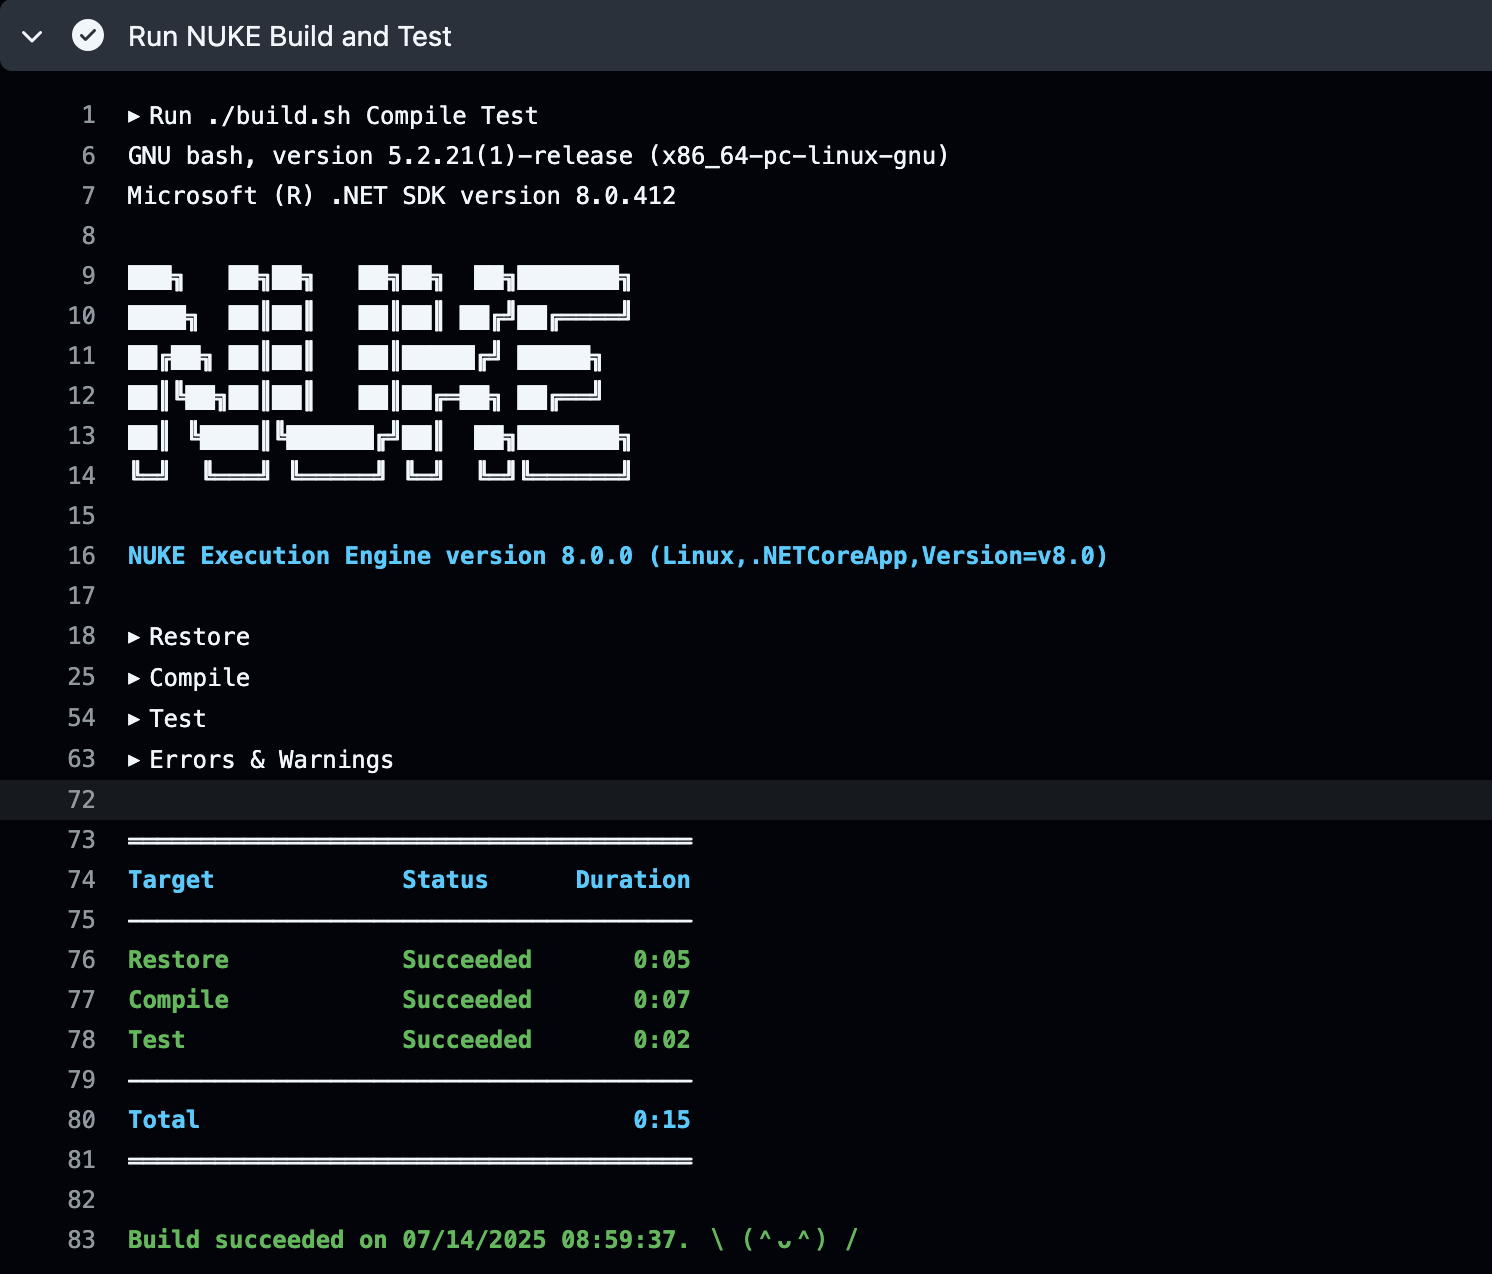
\includegraphics[width=0.4\textwidth]{Nuke-Pipeline.png}
    \end{itemize}
  \columnbreak
    \begin{itemize}
      \item \textbf{CD}
        \begin{itemize}
          \item Github Actions für das Continous-Deployment
          \item Baut eine exe Datei für Windows und eine MacOS App 
        \end{itemize}
        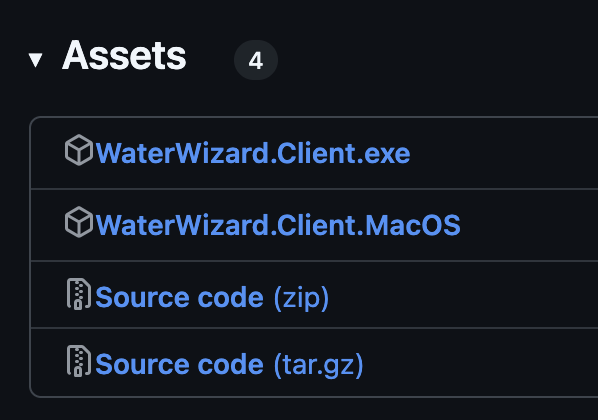
\includegraphics[width=0.4\textwidth]{CD-in-GH.png}
    \end{itemize}
  \end{multicols}
\end{frame}

\subsection{CI-Pipeline Konfiguration}
\begin{frame}[fragile]
\frametitle{CI-Pipeline Konfiguration}
  \begin{lstlisting}[language=yaml, basicstyle=\ttfamily\tiny, breaklines=true]
    name: NUKE Build CI

    on:
      push:
        branches: [ "main", "dev" ] 
      pull_request:
        branches: [ "**" ] 

      workflow_dispatch:

    jobs:
      build:
        runs-on: ubuntu-latest 

        permissions:
          actions: read 
          contents: read 
          security-events: write 

        steps:
          - name: Checkout repository
            uses: actions/checkout@v4
            with:
              fetch-depth: 0 

          - name: Setup .NET SDK
            uses: actions/setup-dotnet@v4
            with:
              dotnet-version: '8.0.x'

          - name: Run NUKE Build and Test
            run: ./build.sh Compile Test
  \end{lstlisting}
\end{frame}

\subsection{CD-Pipeline Konfiguration}
\begin{frame}[fragile]
\frametitle{CD-Pipeline Konfiguration (Teil 1)}
  \begin{lstlisting}[language=yaml, basicstyle=\ttfamily\tiny, breaklines=true]
- name: Publish Client (Windows)
  run: dotnet publish src/WaterWizard.Client/WaterWizard.Client.csproj -c Release -r win-x64 --self-contained true -o ./publish/win --verbosity normal

- name: Publish Server (Windows)
  run: dotnet publish src/WaterWizard.Server/WaterWizard.Server.csproj -c Release -r win-x64 --self-contained true -o ./publish/win-server

- name: Publish Client (MacOS)
  run: dotnet publish src/WaterWizard.Client/WaterWizard.Client.csproj -c Release -r osx-x64 --self-contained true -o ./publish/osx --verbosity normal

- name: Publish Server (MacOS)
  run: dotnet publish src/WaterWizard.Server/WaterWizard.Server.csproj -c Release -r osx-x64 --self-contained true -o ./publish/osx-server

- name: Prepare release assets
  run: |
    mkdir release-assets

    # Find the actual executable names
    WIN_EXE=$(find ./publish/win -name "*.exe" -type f | head -1)
    OSX_EXE=$(find ./publish/osx -type f -executable | grep -v "\.dll$" | grep -v "\.so$" | head -1)
  \end{lstlisting}
\end{frame}

\begin{frame}[fragile]
\frametitle{CD-Pipeline Konfiguration (Teil 2)}
  \begin{lstlisting}[language=yaml, basicstyle=\ttfamily\tiny, breaklines=true]
    if [ -n "$WIN_EXE" ]; then
      cp "$WIN_EXE" release-assets/WaterWizard.Client.exe
    else
      echo "Warning: No Windows executable found"
    fi

    if [ -n "$OSX_EXE" ]; then
      cp "$OSX_EXE" release-assets/WaterWizard.Client.MacOS
    else
      echo "Warning: No MacOS executable found"
    fi

    echo "Release assets:"
    ls -la release-assets/

- name: Create GitHub Release & Upload Assets
  uses: softprops/action-gh-release@v2
  with:
    tag_name: ${{ steps.get_version.outputs.tag }}
    name: Release ${{ steps.get_version.outputs.version }}
    body: ${{ steps.changelog.outputs.changelog }}
    draft: false
    prerelease: false
    files: release-assets/*
  env:
    GITHUB_TOKEN: ${{ secrets.GITHUB_TOKEN }} 
  \end{lstlisting}
\end{frame}

\subsection{Statische Code-Analyse}
\begin{frame}
\frametitle{Statische Code-Analyse}
  \begin{itemize}
    \item CodeQL für die statische Code-Analyse
    \item CodeQL eigene Konfigurationsdatei
      \begin{itemize} 
        \item Möglich auch in der CI Kofigurationsdatei
        \item Best Practice getrennt
        \item Simplere Konfiguration durch seperate Datei
      \end{itemize} 
    \item Ergebnisse in GitHub-Security
  \end{itemize}
\end{frame}

\subsection{CodeQL Konfiguration}
\begin{frame}[fragile]
\frametitle{CodeQL Konfiguration (Teil 1)}
  \begin{lstlisting}[language=yaml, basicstyle=\ttfamily\tiny, breaklines=true]
    name: CodeQL

    on:
      push:
        branches: [ main, dev ]
      pull_request:
        branches: [ '**' ]
      workflow_dispatch:

    jobs:
      analyze:
        name: Analyze
        runs-on: ubuntu-latest
        permissions:
          security-events: write
          actions: read
          contents: read

        strategy:
          fail-fast: false
          matrix:
            language: ['csharp']

        steps:
          - name: Checkout repository
            uses: actions/checkout@v4
            with:
              fetch-depth: 0
  \end{lstlisting}
\end{frame}

\begin{frame}[fragile]
\frametitle{CodeQL Konfiguration (Teil 2)}
  \begin{lstlisting}[language=yaml, basicstyle=\ttfamily\tiny, breaklines=true]
      - name: Setup .NET SDK
            uses: actions/setup-dotnet@v4
            with:
              dotnet-version: '8.0.x'

      - name: Initialize CodeQL
        uses: github/codeql-action/init@v3
        with:
          languages: ${{ matrix.language }}
          config-file: .github/codeql/codeql.yml

      - name: Build with NUKE (required by CodeQL)
        run: ./build.sh Compile

      - name: Perform CodeQL Analysis
        uses: github/codeql-action/analyze@v3
        with:
          category: '/language:${{ matrix.language }}'
  \end{lstlisting}
\end{frame}

\subsection{Containerisierung}
\begin{frame}
\frametitle{Containerisierung}
  \begin{itemize}
    \item Docker für die Containerisierung des Servers
    \item Dockerfile im Server-Verzeichnis
    \item Docker Compose im root-Verzeichnis
  \end{itemize}
\end{frame}

\subsection{Dockerfile Code}
\begin{frame}[fragile]
\frametitle{Dockerfile Code}
  \textbf{Dockerfile}
  \begin{lstlisting}[language=Dockerfile,basicstyle=\ttfamily\tiny]
    FROM mcr.microsoft.com/dotnet/sdk:8.0 AS build
    WORKDIR /source

    COPY WaterWizards.sln .

    COPY src/WaterWizard.Server/WaterWizard.Server.csproj ./src/WaterWizard.Server/
    COPY src/WaterWizard.Shared/WaterWizard.Shared.csproj ./src/WaterWizard.Shared/
    COPY src/WaterWizard.Client/WaterWizard.Client.csproj ./src/WaterWizard.Client/
    COPY src/WaterWizardTests/WaterWizardTests.csproj ./src/WaterWizardTests/

    RUN dotnet restore WaterWizards.sln

    COPY src/WaterWizard.Server/ ./src/WaterWizard.Server/
    COPY src/WaterWizard.Shared/ ./src/WaterWizard.Shared/
    COPY src/WaterWizard.Client/ ./src/WaterWizard.Client/
    COPY src/WaterWizardTests/ ./src/WaterWizardTests/

    RUN dotnet publish src/WaterWizard.Server/WaterWizard.Server.csproj -c Release -o /app/publish

    FROM mcr.microsoft.com/dotnet/runtime:8.0 AS final
    WORKDIR /app

    COPY --from=build /app/publish .


    EXPOSE 7777/udp


    ENTRYPOINT ["dotnet", "WaterWizard.Server.dll"]
  \end{lstlisting}
\end{frame}

\subsection{Docker-Compose Code}
\begin{frame}[fragile]
\frametitle{Docker-Compose Code}
  \textbf{docker-compose}
  \begin{lstlisting}[language=yaml,basicstyle=\ttfamily\tiny]
    version: '3.8'

    services:
      waterwizard-server:
        build:
          context: .
          dockerfile: ./src/WaterWizard.Server/Dockerfile
        ports:
          - "7777:7777/udp"
        environment:
          - PUBLIC_ADDRESS=${SERVER_IP}
  \end{lstlisting}
\end{frame}

\section{Technische Erfahrungen}
\begin{frame}
\frametitle{Technische Erfahrungen}
\end{frame}

\section{Analyse}
\begin{frame}
\frametitle{Analyse}
\begin{columns}
  \begin{column}{1\textwidth}
    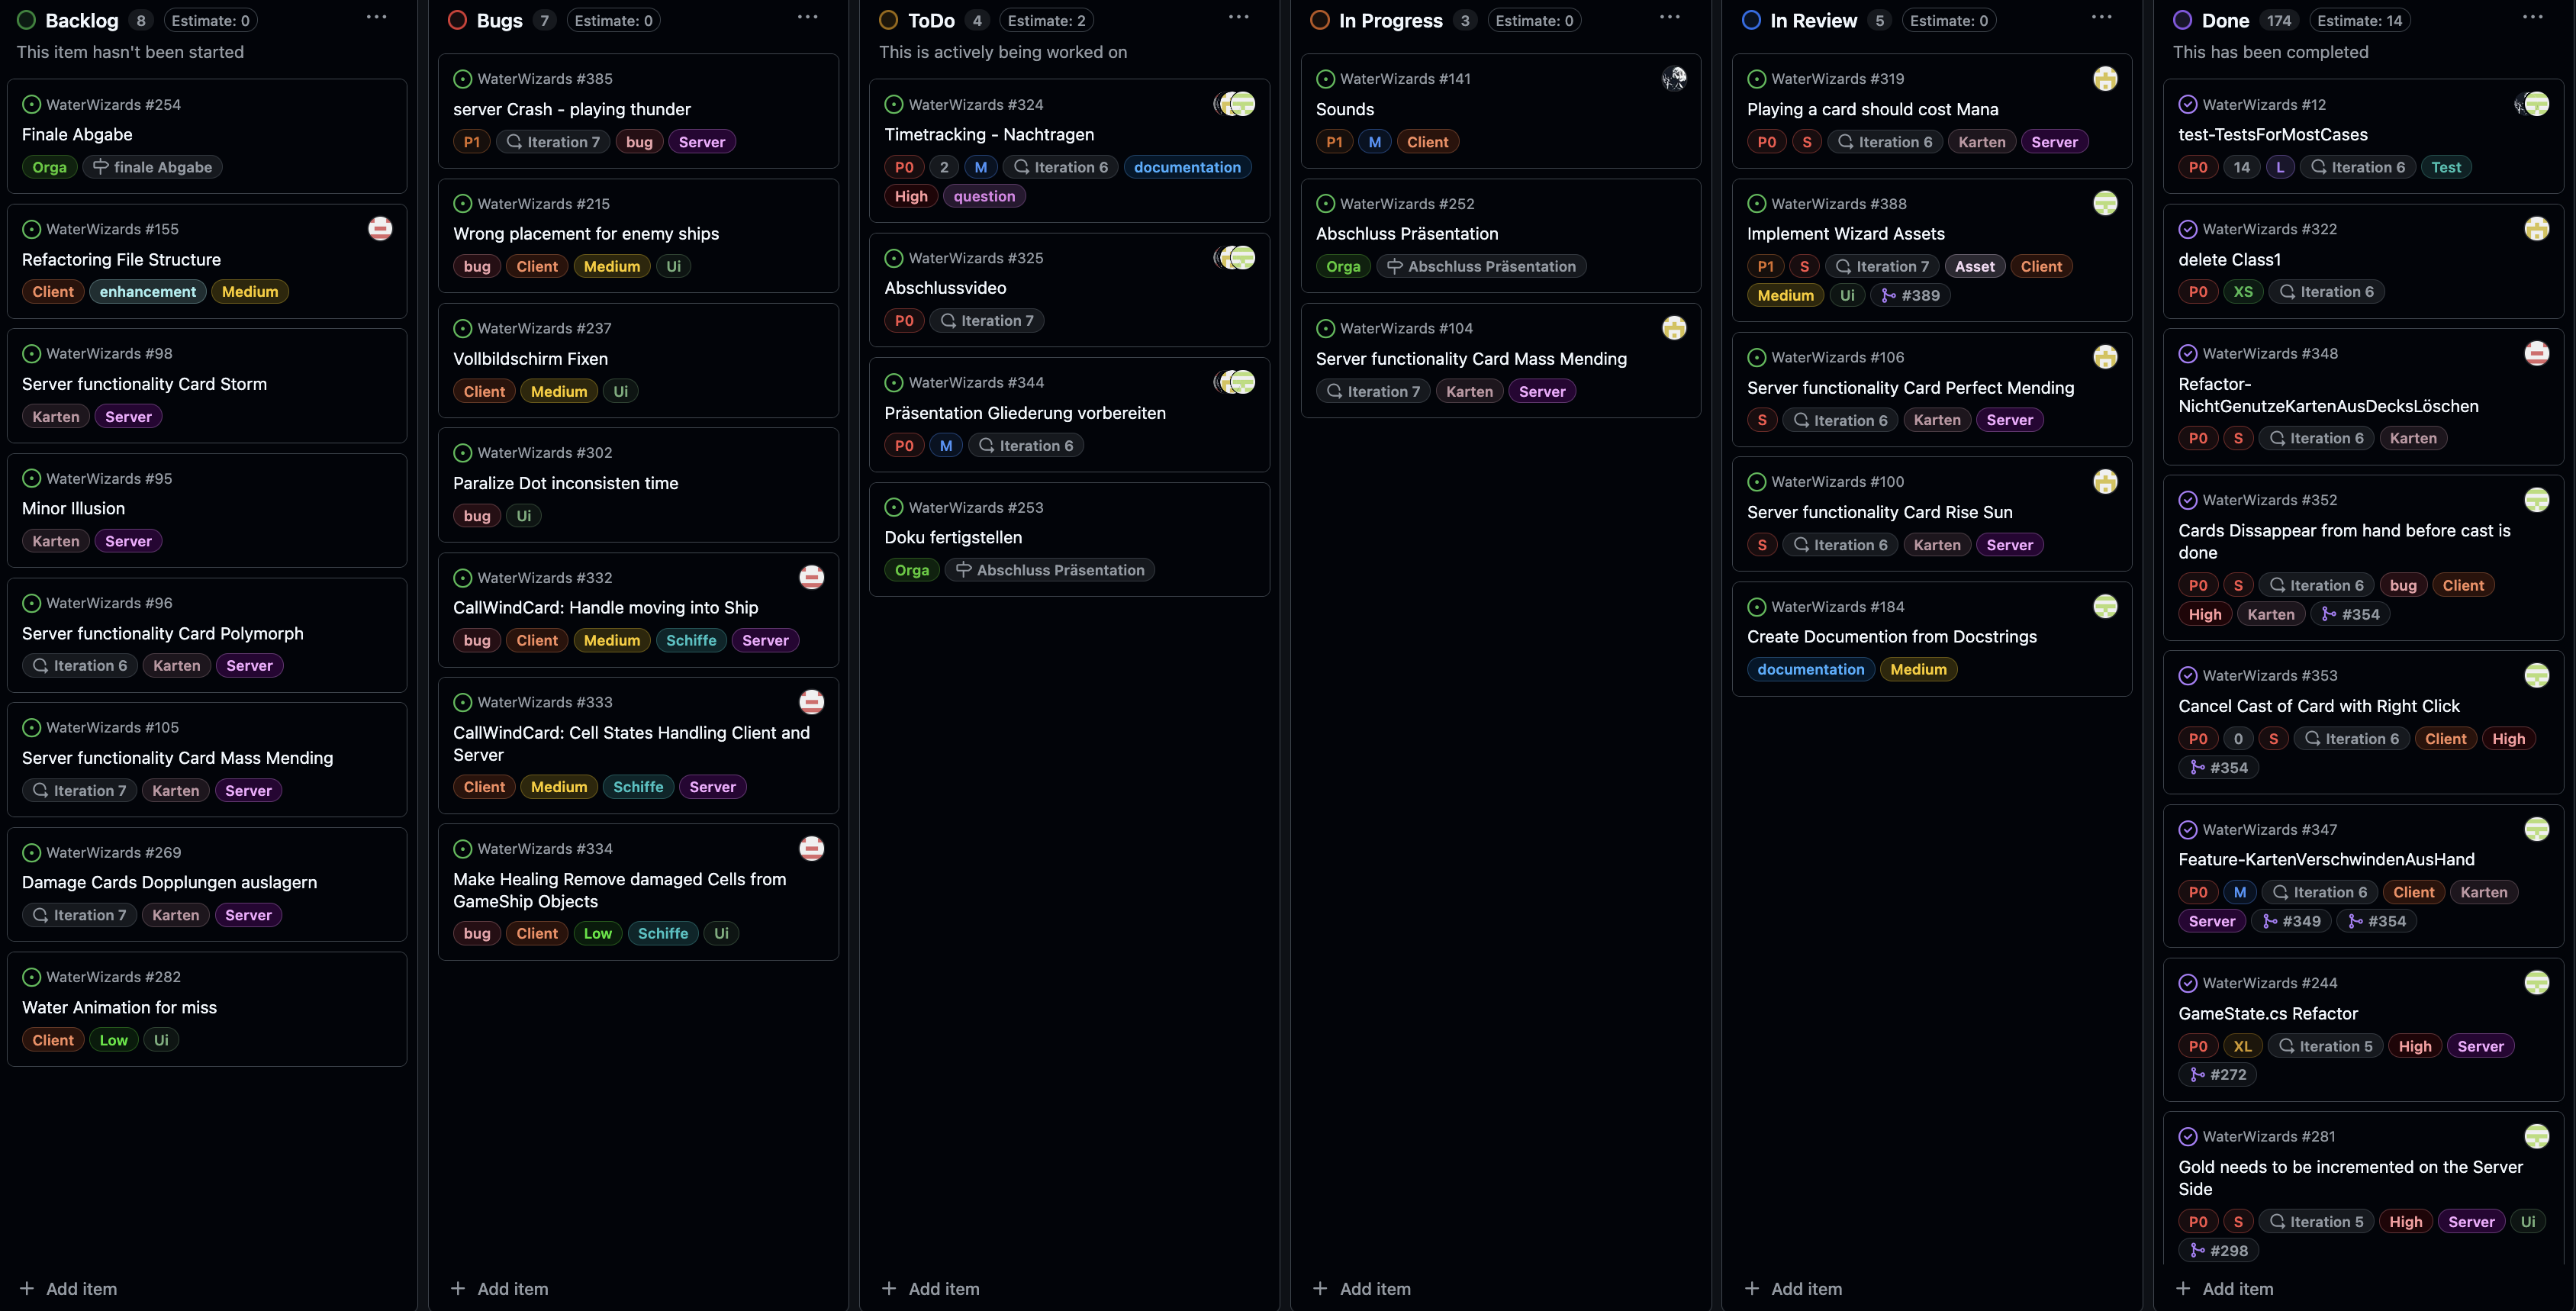
\includegraphics{Kanban.png} % Placeholder for the actual images
  \end{column}
\end{columns}
\end{frame}

\section{Wiki}
\begin{frame}
\frametitle{Wiki}

\end{frame}

\section{Erfahrungen und Fazit}
\begin{frame}
\frametitle{Erfahrungen und Fazit}

\end{frame}


\end{document}